\chapter{आपेक्षिकीय गतिकी}\label{ch:b3:relativistic-dynamics}

1964 में विलियम बर्टोत्सी ने किसी रैखिक त्वरक में दौड़ते इलेक्ट्रॉनों की
फ़िल्म बनाई: हर स्पंद को एक मापी हुई ऊर्जा दी गई, और \qty{8.4}{m} की
उड़ान पर उसकी चाल नापी गई। न्यूटन की भविष्यवाणी थी कि
\qty{15}{MeV} के इलेक्ट्रॉन प्रकाश की चाल से आठ गुना तेज़ उड़ेंगे;
पर विरामघड़ी ने $0.9999c$ बताया और आगे बढ़ने से इनकार कर दिया, चाहे
इलेक्ट्रॉनों को कितना ही ज़ोर से धकेला गया। पिछले अध्याय में शुद्धगतिकी
ने हमें बताया कि $c$ एक सीमा है; अब गतिकी को यह समझाना है कि उस धक्के का
क्या होता है --- जब चाल बढ़नी बंद हो जाए, तब कार्य कहाँ जाता है। उत्तर
यांत्रिकी को एक नए संवेग और एक नई ऊर्जा के चारों ओर फिर से गढ़ देता है,
और दोनों भौतिकी के सबसे प्रसिद्ध समीकरण में जुड़ जाते हैं: संचित ऊर्जा
ही द्रव्यमान है, और द्रव्यमान वहीं बसी ऊर्जा,
$E = mc^2$। यह अध्याय वह गतिकी खड़ी करता है, फिर उसे वहाँ काम पर लगाता
है जहाँ वह रोज़ जीती है --- रेडियोसक्रिय क्षय, कण-संघट्ट, और वे त्वरक
जो गति को नए पदार्थ में बदल देते हैं।

\section{संवेग और ऊर्जा, फिर से गढ़े हुए}

\begin{remark}[$m\vect v$ को क्यों जाना पड़ा]\label{rem:b3:relativistic-dynamics:why}
चिरसम्मत संवेग $m\vect v$ हर तंत्र में संरक्षित रहता है \emph{यदि}
वेग गैलीलियो की रीति से रूपांतरित हों। वे नहीं होते
(\cref{prop:b3:relativistic-kinematics:addition}): जो संघट्ट किसी एक
तंत्र में $\sum m\vect v$ संरक्षित रखता है, वह दूसरे में नहीं रखता, अतः
पुराना संवेग प्रकृति का नियम हो ही नहीं सकता --- अधिक से अधिक किसी नियम
की मंद-चाल छाया। मरम्मत यह है कि वेग को कण की \emph{अपनी} घड़ी से नापा
जाए: $\dd\vect r/\dd\tau =
\gamma\,\vect v$ स्वच्छ रूप से रूपांतरित होता है, और $m\,\dd\vect r/\dd\tau$ सभी तंत्रों में एक साथ संरक्षित
निकलता है।
\end{remark}

\begin{definition}[आपेक्षिकीय संवेग और ऊर्जा]\label{def:b3:relativistic-dynamics:momentum-energy}
\index{आपेक्षिकीय संवेग}\index{आपेक्षिकीय ऊर्जा}\index{विराम ऊर्जा}
द्रव्यमान $m$ और वेग $\vect v$ का कोई कण ($\gamma = 1/\sqrt{1 -
v^2/c^2}$) यह संवेग और यह ऊर्जा वहन करता है
\[
\vect p = \gamma m\vect v , \qquad
E = \gamma mc^2 .
\]
विराम में $E_0 = mc^2$: यही \emph{विराम ऊर्जा} है। गतिज ऊर्जा वह है जो
गति जोड़ती है, $E_k = E - mc^2 = (\gamma - 1)mc^2$, जो $v
\ll c$ के लिए घटकर परिचित $\tfrac12 mv^2$ रह जाती है ($\gamma$ का
प्रसार कीजिए)। हर विलगित प्रक्रिया में कुल $\vect p$ और कुल $E$ ---
विराम ऊर्जाएँ सहित --- संरक्षित रहते हैं।
\end{definition}

\begin{theorem}[ऊर्जा--संवेग संबंध]\label{thm:b3:relativistic-dynamics:relation}
\index{ऊर्जा--संवेग संबंध}
किसी भी कण के लिए,
\[
E^2 = (pc)^2 + (mc^2)^2 ,
\qquad
\vect v = \frac{\vect p\,c^2}{E} :
\]
संयोजन $E^2 - p^2c^2 = m^2c^4$ का मान हर तंत्र में एक ही रहता है ---
ऊर्जा और संवेग के लिए वह वही है जो काल और दिक् के लिए अंतराल है।
दो परिसर: नीची चाल पर $E \approx mc^2 + p^2/2m$; और
ऊँची ऊर्जा पर ($E \gg mc^2$) $E \approx pc$ तथा $v \to c$: और ज़ोर से
धकेलने से ऊर्जा और संवेग बढ़ते हैं, चाल लगभग नहीं।
\end{theorem}

\begin{proof}
$E^2 - p^2c^2 = \gamma^2m^2c^4(1 - v^2/c^2) = m^2c^4$; और $pc^2/E =
\gamma mvc^2/\gamma mc^2 = v$। तंत्र-निश्चरता इसलिए निकलती है कि $m$
और $c$ तंत्र-निरपेक्ष हैं।
\end{proof}

\begin{proposition}[द्रव्यमानहीन कण]\label{prop:b3:relativistic-dynamics:massless}
\index{फ़ोटॉन!संवेग}
शून्य द्रव्यमान वाले कण का $E = pc$ होता है और वह हर तंत्र में ठीक
$c$ से चलता है; उसे धीमा नहीं किया जा सकता, केवल लाल-विस्थापित। फ़ोटॉन
इसका मानक उदाहरण है: $E = h\nu$ और $p = h\nu/c = h/\lambda$ ---
वर्ष 1 के खंड के प्लांक--आइंस्टाइन संबंध, जिन्हें अब यांत्रिकी के
$m = 0$ वाले कोने के रूप में देखा जाता है।
\end{proposition}

\begin{proof}
\cref{thm:b3:relativistic-dynamics:relation} में $m = 0$ रखिए: $E = pc$
और $v = pc^2/E = c$।
\end{proof}

\begin{omfigure}
\begin{tikzpicture}
  \begin{axis}[omaxis, axis x line=bottom, axis y line=left,
    width=6.6cm, height=5.4cm, xmin=0, xmax=4.3, ymin=0, ymax=1.35,
    xlabel={$E_k/mc^2$}, ylabel={$v^2/c^2$},
    xlabel style={at={(axis description cs:0.5,-0.1)}, anchor=north},
    xtick={1,2,3,4}, ytick={0.5,1}, clip=false]
    \addplot[omExo, dashed, thick, domain=0:0.68] {2*x};
    \addplot[omDef, very thick, domain=0:4.3, samples=80] {1 - 1/(1+x)^2};
    \addplot[gray, dashed, domain=0:4.3] {1};
    \node[omExo, font=\scriptsize, anchor=west] at (axis cs:0.8,1.24) {न्यूटन: $v^2 = 2E_k/m$};
    \node[omDef, font=\scriptsize, anchor=west] at (axis cs:2.0,0.82) {आपेक्षिकता};
    \fill[omThm] (axis cs:0.87,0.714) circle (1.6pt);
    \fill[omThm] (axis cs:1.96,0.886) circle (1.6pt);
    \fill[omThm] (axis cs:2.94,0.935) circle (1.6pt);
  \end{axis}
  \begin{axis}[omaxis, axis x line=bottom, axis y line=left,
    width=6.6cm, height=5.4cm, xmin=0, xmax=3, ymin=0, ymax=3.3,
    xshift=7.2cm,
    xlabel={$pc/mc^2$}, ylabel={$E/mc^2$},
    xlabel style={at={(axis description cs:0.5,-0.1)}, anchor=north},
    xtick={1,2,3}, ytick={1,2,3}, clip=false]
    \addplot[omDef, very thick, domain=0:3, samples=60] {sqrt(1+x*x)};
    \addplot[omExo, dashed, domain=0:3] {x};
    \draw[<->, omThm] (axis cs:0,0.04) -- (axis cs:0,0.96);
    \node[omThm, font=\scriptsize, anchor=west] at (axis cs:0.06,0.5) {$mc^2$};
    \node[omExo, font=\scriptsize, anchor=north west] at (axis cs:2.1,2.0) {$E = pc$ (प्रकाश)};
    \node[omDef, font=\scriptsize, anchor=south east] at (axis cs:2.9,3.1) {$E = \sqrt{p^2c^2 + m^2c^4}$};
  \end{axis}
\end{tikzpicture}

{\small बाएँ: बर्टोत्सी का ``परम चाल'' प्रयोग --- नापी गई
इलेक्ट्रॉन-चालें (बिंदु) आपेक्षिकीय वक्र का अनुसरण करती हैं और
$c$ पर संतृप्त हो जाती हैं, जबकि न्यूटन की रेखा उससे परे निकल जाती है।
दाएँ: ऊर्जा--संवेग अतिपरवलय; $p = 0$ पर उसका अंतःखंड \omterm{def:b3:relativistic-dynamics:momentum-energy}{विराम ऊर्जा} है, और
उसका अनंतस्पर्शी फ़ोटॉन का $E = pc$।}
\end{omfigure}

\begin{example}[परिमाण की कोटियाँ]\label{ex:b3:relativistic-dynamics:orders}
कण-भौतिकी ऊर्जा को इलेक्ट्रॉनवोल्ट में और द्रव्यमानों को
$\unit{MeV}/c^2$ में गिनती है: इलेक्ट्रॉन $0.511$, प्रोटॉन $938.3$,
म्युऑन $105.7$, पायॉन $139.6$। \qty{1}{MeV} गतिज ऊर्जा वाले किसी
इलेक्ट्रॉन का $\gamma =
2.96$ और $v = 0.94c$ होता है --- अर्थात् वह
पहले से ही पूरी तरह आपेक्षिकीय है, और इसीलिए इलेक्ट्रॉनिकी चिरसम्मत
बनी रहती है (\unit{eV}) जबकि नाभिकीय भौतिकी नहीं
(\unit{MeV})। \qty{6.8}{TeV} के किसी LHC प्रोटॉन का $\gamma = 7250$ है
और वह किसी फ़ोटॉन से केवल \qty{2.9}{m/s} पीछे रहता है।
\end{example}

\section{द्रव्यमान वहीं बसी ऊर्जा है}

\begin{theorem}[द्रव्यमान--ऊर्जा तुल्यता]\label{thm:b3:relativistic-dynamics:emc2}
\index{द्रव्यमान--ऊर्जा तुल्यता}\index{द्रव्यमान क्षति}
किसी पिंड का द्रव्यमान उसकी अंतर्वस्तु की कुल ऊर्जा है, जिसे
$c^2$ से भाग दिया गया हो और उसके विराम-तंत्र में नापा गया हो: पिंड को
गरम कीजिए, उसकी स्प्रिंग कसिए, उसके परमाणु उत्तेजित कीजिए --- वह
$\Delta E/c^2$ जितना भारी हो जाएगा; उसके भागों को बाँध दीजिए और वह
बंधन ऊर्जा को $c^2$ से भाग देने जितना \emph{हलका} हो जाएगा --- यही
\emph{\omterm{thm:b3:relativistic-dynamics:emc2}{द्रव्यमान क्षति}} है। और उलटे, \omterm{def:b3:relativistic-dynamics:momentum-energy}{विराम ऊर्जा} मुक्त भी की जा सकती है:
जब भी अंतिम द्रव्यमानों का योग आरंभिक से कम हो, तब
अंतर $\Delta m\,c^2$ गतिज ऊर्जा या विकिरण के रूप में निकल आता है।
\end{theorem}
\admitted

\begin{example}[$c^2$ का बहीखाता]\label{ex:b3:relativistic-dynamics:ledger}
$c^2 = \qty{9e16}{J/kg}$: द्रव्यमान का एक ग्राम अंतर
\qty{9e13}{J} है, अर्थात् किसी छोटे नगर की एक दिन की ऊर्जा। रासायनिक
बंध (प्रति अणु कुछ eV) द्रव्यमानों को $10^{10}$ में एक भाग जितना
खिसकाते हैं --- सदा के लिए अतौल्य, और इसीलिए रसायन ने कभी ध्यान नहीं
दिया। नाभिकीय बंधन उन्हें लगभग $1\%$ जितना खिसका देता है: हीलियम अपने
चार हाइड्रोजन अवयवों से $0.7\%$ हलका है, और वही लुप्त अंश, सूर्य से
प्रकाश के रूप में बहता हुआ, उसे हर सेकंड $\Delta m = L_\odot/c^2 =
\qty{4.3e9}{kg}$ का पड़ता है --- चालीस लाख टन धूप। विनाशन पूरा
हिसाब चुका देता है: किसी पॉज़िट्रॉन से मिलता इलेक्ट्रॉन
\qty{511}{keV} के दो फ़ोटॉनों के सिवा कुछ नहीं छोड़ता, और यही वह संकेत
है जिससे PET क्रमवीक्षक किसी जीवित मस्तिष्क को देखते हैं।
\end{example}

\begin{remark}[``परिवर्तन'' का अर्थ क्या है]\label{rem:b3:relativistic-dynamics:conversion}
कोई भी भौतिक वस्तु ऊर्जा में ``बदल'' नहीं जाती: कुल ऊर्जा तो शुरू से
संरक्षित थी। जो बदलता है वह उसका \emph{निवास} है --- \omterm{def:b3:relativistic-dynamics:momentum-energy}{विराम ऊर्जा} से,
जो तौल में आती है, गतिज ऊर्जा और विकिरण तक, जो उड़ जाते हैं।
$E = mc^2$ का गहरा कथन यह है कि जड़त्व स्वयं एक ऊर्जा-अंतर्वस्तु है:
गरम गैस से भरा संदूक उसी ठंडे संदूक से अधिक त्वरण का प्रतिरोध करता है।
\end{remark}

\section{संघट्ट और क्षय}

\begin{definition}[चतुःसंवेग और निश्चर द्रव्यमान]\label{def:b3:relativistic-dynamics:four-momentum}
\index{चतुःसंवेग}\index{निश्चर द्रव्यमान}
किसी कण की ऊर्जा और संवेग को उसके \emph{चतुःसंवेग}
$P = (E/c, \vect p)$ में बाँध दीजिए। कणों के किसी निकाय के लिए घटकवार
जोड़िए: $E_{\text{कुल}} = \sum E_i$, $\vect p_{\text{कुल}} = \sum\vect p_i$।
निकाय का \emph{निश्चर द्रव्यमान} $M$ इस तरह परिभाषित है
\[
M^2c^4 = E_{\text{कुल}}^2 - \|\vect p_{\text{कुल}}\|^2c^2 :
\]
यह हर तंत्र में एक ही संख्या है, और उस \emph{संवेग-केंद्र तंत्र} की
कुल ऊर्जा ($c^2$ से भाग देने पर) के बराबर है जिसमें
$\vect p_{\text{कुल}} = \vect 0$ हो। ध्यान दीजिए कि जब भी भाग एक-दूसरे
के सापेक्ष चलते हैं, तब $M$ उनके द्रव्यमानों के योग से अधिक होता है ---
अलग-अलग उड़ते दो फ़ोटॉनों का $M > 0$ होता है, यद्यपि हर एक द्रव्यमानहीन है।
\end{definition}

\begin{method}[किसी आपेक्षिकीय संघट्ट को हल करना]\label{met:b3:relativistic-dynamics:method}
(1) \omterm{def:b3:relativistic-dynamics:four-momentum}{चतुःसंवेग} का संरक्षण लिखिए: $E$ और $\vect p$ साथ-साथ,
कभी अकेला नहीं। (2) जिस भी बंडल की सुविधा हो, उसका निश्चर
$E^2 - p^2c^2$ निकालिए --- उसका मान सबसे आसान तंत्र में निकाला जा सकता
है और किसी भी दूसरे में काम में लाया जा सकता है। (3) देहलियाँ: कोई
अभिक्रिया तब संभव है जब आरंभिक अवस्था का \omterm{def:b3:relativistic-dynamics:four-momentum}{निश्चर द्रव्यमान} अंतिम अवस्था
के विराम-द्रव्यमानों के योग तक पहुँच जाए। (4) विराम में क्षय: उत्पादों
के संवेग विपरीत और बराबर होते हैं; ऊर्जाएँ केवल द्रव्यमानों से निकल
आती हैं। (5) चालों में बदलना, यदि पूछा जाए, तो सबसे अंत में ही, $v = pc^2/E$ से।
\end{method}

\begin{example}[पायॉन की छाप]\label{ex:b3:relativistic-dynamics:pion}
विराम में कोई आवेशित पायॉन क्षय होता है, $\pi^+ \to \mu^+ + \nu$
(न्यूट्रिनो व्यावहारिक रूप से द्रव्यमानहीन)। संवेग-संरक्षण उत्पादों को
बराबर $p$ के साथ आमने-सामने भेज देता है; ऊर्जा-संरक्षण कहता है $m_\pi c^2 =
\sqrt{p^2c^2 + m_\mu^2c^4} + pc$। हल करने पर:
\[
pc = \frac{(m_\pi^2 - m_\mu^2)c^2}{2m_\pi} = \qty{29.8}{MeV} ,
\]
अर्थात् विराम में क्षय होते किसी पायॉन से निकला हर म्युऑन ठीक
\qty{4.1}{MeV} गतिज ऊर्जा के साथ जन्मता है --- एक एकऊर्जीय रेखा, और
उसका प्रेक्षण (पॉवेल, 1947) ही वह तरीका था जिससे पायॉन का द्रव्यमान
पहली बार तौला गया। द्वि-पिंड क्षय सदा ऐसी रेखाएँ देते हैं; त्रि-पिंड
क्षय उन्हें वर्णक्रमों में फैला देते हैं, और ठीक इसी से नाभिकीय
$\beta$ क्षय में न्यूट्रिनो का पहला संदेह हुआ था।
\end{example}

\begin{proposition}[देहलियाँ: नियत लक्ष्य का अत्याचार]\label{prop:b3:relativistic-dynamics:threshold}
\index{देहली ऊर्जा}\index{संघट्टक}
नए कण बनाने के लिए केवल \emph{संवेग-केंद्र} की ऊर्जा
$Mc^2$ उपलब्ध होती है। ऊर्जा $E$ का कोई पुंज, जो विराम में रखे
द्रव्यमान $m_{\text{t}}$ के लक्ष्य से टकराए, यह देता है
\[
M^2c^4 = m_{\text{b}}^2c^4 + m_{\text{t}}^2c^4 +
2\,E\,m_{\text{t}}c^2 :
\]
उपयोगी ऊर्जा केवल $\sqrt E$ की तरह बढ़ती है --- बाकी मलबे को आगे
धकेलने में बरबाद हो जाती है। आमने-सामने टकराते दो सर्वसम पुंज
$Mc^2 = 2E$ देते हैं: पूरा का पूरा उपयोगी। यही एक सूत्र है जिसके कारण
सीमांत की मशीनें संघट्टक हैं
(\cref{pb:b3:relativistic-dynamics:1})।
\end{proposition}

\begin{proof}
प्रयोगशाला में $E_{\text{कुल}}^2 - p_{\text{कुल}}^2c^2$ का मान निकालिए:
$(E + m_{\text{t}}c^2)^2 - p^2c^2$, जहाँ $p$ पुंज का संवेग है; प्रसार
कीजिए और $E^2 - p^2c^2 = m_{\text{b}}^2c^4$ काम में लाइए। संघट्टक के लिए
$\vect p_{\text{कुल}} = \vect 0$ और $Mc^2 = E_{\text{कुल}}$।
\end{proof}

\begin{omfigure}
\begin{tikzpicture}[font=\small, >=Stealth]
  % fixed target
  \begin{scope}
    \fill[omDef] (0,0) circle (2.6pt);
    \draw[->, omDef, very thick] (0.15,0) -- (1.45,0);
    \node[font=\footnotesize] at (0.0,0.42) {$E$};
    \fill[omExo] (2.3,0) circle (2.6pt);
    \node[font=\footnotesize] at (2.3,0.42) {विराम में};
    \draw[->, thick] (3.1,0) -- (3.8,0);
    \fill[gray] (4.6,0) circle (2.6pt);
    \draw[->, gray, very thick] (4.75,0) -- (5.9,0);
    \draw[->, gray, thick] (4.68,0.12) -- (5.5,0.62);
    \draw[->, gray, thick] (4.68,-0.12) -- (5.5,-0.62);
    \node[align=center, font=\footnotesize] at (2.9,-1.25)
      {नियत लक्ष्य: $Mc^2 \approx \sqrt{2\,E\,m_{\text{t}}c^2}$\\मलबा अधिकांश ऊर्जा रख लेता है};
  \end{scope}
  % collider
  \begin{scope}[xshift=8.3cm]
    \fill[omDef] (0,0) circle (2.6pt);
    \draw[->, omDef, very thick] (0.15,0) -- (1.45,0);
    \node[font=\footnotesize] at (0.0,0.42) {$E$};
    \fill[omThm] (3.4,0) circle (2.6pt);
    \draw[->, omThm, very thick] (3.25,0) -- (1.95,0);
    \node[font=\footnotesize] at (3.4,0.42) {$E$};
    \node[align=center, font=\footnotesize] at (1.7,-1.25)
      {संघट्टक: $Mc^2 = 2E$\\हर जूल उपलब्ध है};
  \end{scope}
\end{tikzpicture}

{\small गति से पदार्थ बनाना: नियत लक्ष्य पर संवेग-संरक्षण उत्पादों को
उड़ते रहने पर विवश कर देता है, और उपयोगी
संवेग-केंद्र ऊर्जा केवल $\sqrt E$ की तरह बढ़ती है; आमने-सामने के
संघट्ट में वह पूरी $2E$ होती है।}
\end{omfigure}

\section{बल और मशीनें}

\begin{proposition}[आपेक्षिकीय गति-समीकरण]\label{prop:b3:relativistic-dynamics:force}
\index{सिंक्रोट्रॉन}
न्यूटन का नियम इस रूप में बचा रहता है
\[
\vect F = \frac{\dd\vect p}{\dd t} = \frac{\dd(\gamma m\vect v)}
{\dd t} , \qquad
\frac{\dd E}{\dd t} = \vect F\cdot\vect v .
\]
कोई चुंबकीय क्षेत्र, जो सदा $\vect v$ के लंबवत रहता है, ऊर्जा नहीं
बदलता और प्रक्षेप-पथ को इस त्रिज्या के वृत्त में मोड़ देता है
\[
r = \frac{p}{qB}
\]
--- वही सूत्र जो वर्ष 1 के खंड में था, पर आपेक्षिकीय
$p$ के साथ। पर परिक्रमण-आवृत्ति $qB/\gamma m$ अब कण की ऊर्जा बढ़ने के
साथ \emph{घटती} है: साइक्लोट्रॉन का नियत-आवृत्ति धक्का MeV पैमाने के
पास ताल से बाहर हो जाता है, और उच्च-ऊर्जा मशीनें ---
\emph{सिंक्रोट्रॉन} --- इसके बदले अपना क्षेत्र और अपनी आवृत्ति
$\gamma$ के साथ ताल में बढ़ाती जाती हैं, और पुंज को एक ही वलय पर रखे
रहती हैं।
\end{proposition}

\begin{proof}[आंशिक उपपत्ति]
बल-नियम नए संवेग के अनुरूप गतिकी की परिभाषा ही है
($\dd E/\dd t$, $E^2 = p^2c^2 + m^2c^4$ से निकलता है:
$E\,\dot E = c^2\vect p\cdot\dot{\vect p}$)।
वृत्त के लिए: $|\dd\vect p/\dd t| = qvB$, जबकि $|\vect p|$ अचर है, का
अर्थ है कि संवेग-सदिश $qvB/p$ दर से घूमता है, अतः त्रिज्या
$v/(qvB/p) = p/qB$ है।
\end{proof}

\begin{example}[LHC को किसी अभ्यास की तरह पढ़ना]\label{ex:b3:relativistic-dynamics:lhc}
$E = \qty{6.8}{TeV}$ के प्रोटॉन, $B = \qty{8.3}{T}$ के द्विध्रुवों में:
$p \approx E/c$ (अति-आपेक्षिकीय), अतः $r = p/qB =
\qty{2.7}{km}$ --- और सचमुच वलय की चुंबकीय मोड़-त्रिज्या
\qty{2.8}{km} है, क्योंकि \qty{27}{km} की परिधि का अधिकांश चुंबक ही
है। आमने-सामने के संघट्ट $Mc^2 = \qty{13.6}{TeV}$ देते हैं; नियत लक्ष्य
पर उतना पाने के लिए $2E^2/m_{\text{p}}c^2 \approx
\qty{e17}{eV}$ का पुंज चाहिए --- अब तक बनी किसी भी मशीन की पहुँच से सौ
गुना अधिक। आधुनिक ऊर्जा-सीमांत प्रबल चुंबकों ने नहीं, संघट्टक के सूत्र
ने खरीदा है।
\end{example}

\begin{omfigure}
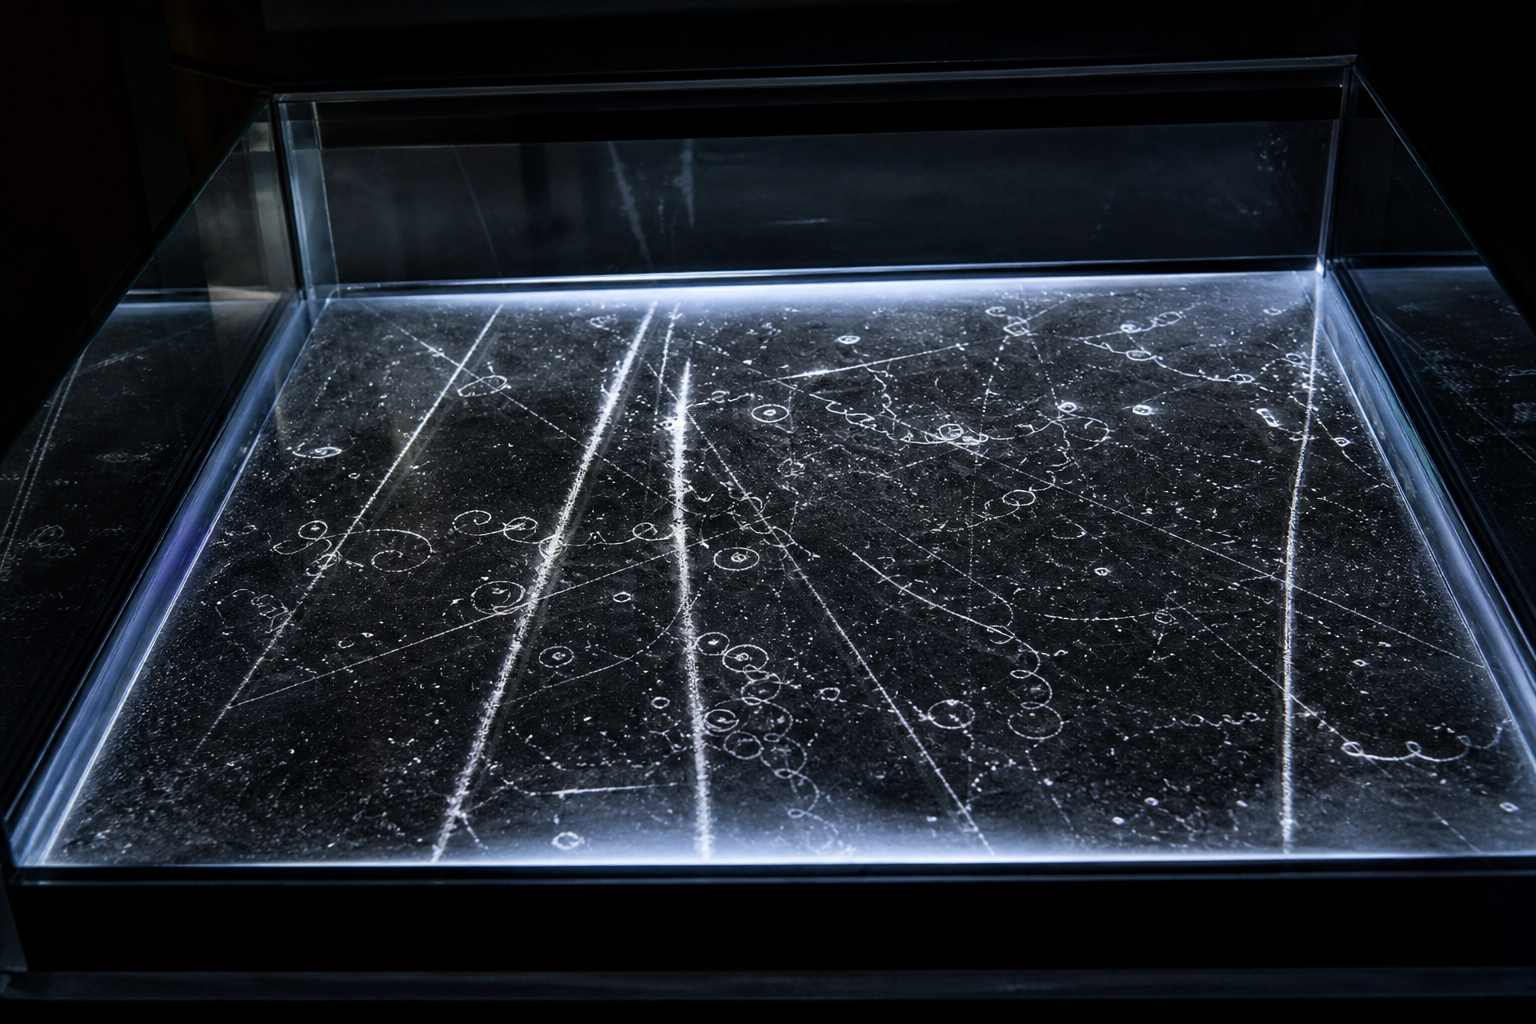
\includegraphics[width=0.58\linewidth]{images/book5/ai/b5-05-cloud-chamber.png}

{\small कुहरा-कक्ष को पार करते आवेशित कण। ऐसे ही चिह्न --- चुंबकीय क्षेत्रों में मुड़ते हुए, युग्मों में प्रकट होते हुए --- ने $E = mc^2$ को सूत्र से रोज़ के बहीखाते में बदल दिया: पॉज़िट्रॉन की खोज ऐसे ही किसी छायाचित्र पर हुई थी।}
\end{omfigure}

\section{अभ्यास}

\begin{exercise}[$\star$]\label{exo:b3:relativistic-dynamics:1}
कोई इलेक्ट्रॉन ($mc^2 = \qty{0.511}{MeV}$) $0.99c$ से चलता है।
$\gamma$, उसका संवेग $\unit{MeV}/c$ में, तथा उसकी कुल और गतिज
ऊर्जाएँ निकालिए। वही प्रश्न \qty{1}{GeV} गतिज ऊर्जा वाले किसी
प्रोटॉन ($mc^2 = \qty{938}{MeV}$) के लिए।
\end{exercise}

\begin{exercise}[$\star$]\label{exo:b3:relativistic-dynamics:2}
(क) एक ग्राम पदार्थ में कितनी ऊर्जा सोई हुई है? (ख) हिरोशिमा के
विस्फोट ने लगभग \qty{6e13}{J} मुक्त की: वह कितना द्रव्यमान-अंतर है?
(ग) सूर्य $L = \qty{3.8e26}{W}$ विकिरित करता है: वह प्रति सेकंड कितना
द्रव्यमान छोड़ता है, और दस अरब वर्षों में अपने $\qty{2e30}{kg}$ का
कितना अंश? (घ) आपके फ़ोन की बैटरी \qty{5e4}{J} संचित रखती है: चार्ज
किया हुआ फ़ोन कितना भारी होता है?
\end{exercise}

\begin{exercise}[$\star$]\label{exo:b3:relativistic-dynamics:3}
(क) \qty{5}{mW} के किसी लेज़र-सूचक का पुंज प्रति सेकंड कितना संवेग ले
जाता है, और सूचक को कितना बल अनुभव होता है? (ख) धूप
(\qty{1.4}{kW/m^2}) पूर्णतः परावर्तक \qty{100}{m^2} की किसी सौर-पाल
पर कितना बल लगाती है? (ग) विराम से चलकर \qty{10}{kg} का कोई
पाल-यान एक महीने बाद कितनी तेज़ी से चल रहा होगा? (घ) किसी धूमकेतु की
धूल-पूँछ सूर्य से दूर की ओर क्यों संकेत करती है?
\end{exercise}

\begin{exercise}[$\star$]\label{exo:b3:relativistic-dynamics:4}
मात्रकों का अभ्यास। (क) दिखाइए कि $\unit{MeV}/c^2$ द्रव्यमान का
मात्रक है, और इलेक्ट्रॉन का द्रव्यमान किलोग्राम में बदलिए। (ख)
$\unit{kg.m/s}$ में \qty{1}{GeV/c} कितना है? (ग) किसी \omterm{def:b3:relativistic-dynamics:four-momentum}{निश्चर द्रव्यमान}
का वर्ग $s = \qty{16}{GeV^2}$ निकलता है ($c = 1$ मात्रकों में): वह
कितनी संवेग-केंद्र ऊर्जा है? (घ) कण-भौतिक
$c = 1$ क्यों रखते हैं, और SI संख्याएँ पाने के लिए पाठक को क्या फिर से
डालना पड़ता है?
\end{exercise}

\begin{exercise}[$\star\star$]\label{exo:b3:relativistic-dynamics:5}
बर्टोत्सी के इलेक्ट्रॉनों की गतिज ऊर्जाएँ $0.5$, $1$, $4.5$ और
\qty{15}{MeV} थीं। (क) हर एक के लिए न्यूटन की भविष्यवाणी $v^2 = 2E_k/m$
निकालिए, $c^2$ के मात्रकों में। (ख) आपेक्षिकीय $v^2/c^2$ निकालिए। (ग)
\qty{15}{MeV} पर \qty{8.4}{m} का उसका उड़ान-काल: घड़ी ने क्या पढ़ा, और
न्यूटन ने क्या भविष्यवाणी की होती? (घ) इलेक्ट्रॉनों की ऊर्जा
कैलोरीमिति से भी नापी गई थी --- टकराने पर उनकी ऊष्मा से:
वही कदम इस प्रयोग का असली मर्म क्यों था?
\end{exercise}

\begin{exercise}[$\star\star$]\label{exo:b3:relativistic-dynamics:6}
आवेशित पायॉन विराम में क्षय होता है: $\pi^+ \to \mu^+\nu$, $m_\pi c^2 =
\qty{139.6}{MeV}$, $m_\mu c^2 = \qty{105.7}{MeV}$, $m_\nu \approx 0$।
(क) दिखाइए कि $pc = (m_\pi^2 - m_\mu^2)c^4/2m_\pi c^2$ और उसका मान
निकालिए। (ख) म्युऑन की गतिज ऊर्जा और चाल। (ग) न्यूट्रिनो की ऊर्जा।
(घ) $\gamma_\pi = 50$ पर उड़ते हुए क्षय में, क्षय-म्युऑन की अधिकतम और
न्यूनतम प्रयोगशाला-ऊर्जाएँ क्या हैं (आगे और पीछे की ओर क्षय)?
\end{exercise}

\begin{exercise}[$\star\star$]\label{exo:b3:relativistic-dynamics:7}
\omterm{def:b3:relativistic-dynamics:four-momentum}{निश्चर द्रव्यमान}, काम पर। (क) \qty{200}{MeV} के दो फ़ोटॉन एक-दूसरे से
$60^\circ$ पर उड़ते हैं: युग्म का \omterm{def:b3:relativistic-dynamics:four-momentum}{निश्चर द्रव्यमान} निकालिए।
(ख) कोई उदासीन पायॉन ($m_{\pi^0}c^2 = \qty{135}{MeV}$) दो फ़ोटॉनों में
क्षय होता है: हर तंत्र में उस फ़ोटॉन-युग्म का \omterm{def:b3:relativistic-dynamics:four-momentum}{निश्चर द्रव्यमान} क्या
है? (ग) समझाइए कि कोई प्रयोग किसी कण को उसके क्षय-उत्पादों के
निश्चर-द्रव्यमान बंटन में एक उभार के रूप में कैसे ``खोजता'' है। (घ)
बराबर ऊर्जा के दो फ़ोटॉन ठीक समांतर उड़ते हैं: \omterm{def:b3:relativistic-dynamics:four-momentum}{निश्चर द्रव्यमान}?
इससे किसी प्रकाश-पुंज के विराम-तंत्र के विषय में क्या पता चलता है?
\end{exercise}

\begin{exercise}[$\star\star$]\label{exo:b3:relativistic-dynamics:8}
LHC का बहीखाता ($E = \qty{6.8}{TeV}$ के प्रोटॉन)। (क) $\gamma$, और
चाल की कमी $c - v$ ($c - v \approx c/2\gamma^2$ काम में लाइए)। (ख)
\qty{27}{km} के वलय पर परिक्रमण-आवृत्ति और प्रति सेकंड चक्करों की
संख्या। (ग) \num{3e14} प्रोटॉनों के पुंज की संचित ऊर्जा,
TNT (\qty{4.2e6}{J/kg}) के किलोग्रामों में। (घ) दोनों पुंजों की गतिज
ऊर्जा का द्रव्यमान-तुल्य, माइक्रोग्राम में --- वह पदार्थ जो अभी बनने वाला है।
\end{exercise}

\begin{exercise}[$\star\star$]\label{exo:b3:relativistic-dynamics:9}
टकराते फ़ोटॉन। (क) दिखाइए कि निर्वात में कोई अकेला फ़ोटॉन किसी
इलेक्ट्रॉन--पॉज़िट्रॉन युग्म में क्षय नहीं हो सकता, चाहे कितना ही
ऊर्जावान हो (निश्चर काम में लाइए)। (ख) ऊर्जा $\epsilon$ के किसी दूसरे
फ़ोटॉन से आमने-सामने टकराने पर दिखाइए कि युग्म-सृजन के लिए
$E\epsilon \ge (m_{\text{e}}c^2)^2$ चाहिए। (ग) किसी
\qty{511}{keV} फ़ोटॉन को कैसा साथी चाहिए? \qty{50}{keV} की किसी
एक्स-किरण को? (घ) ब्रह्मांड तारों के प्रकाश और ब्रह्मांडीय सूक्ष्मतरंग
पृष्ठभूमि से भरा है: (ख) अंतर-मंदाकिनीय दिक् में TeV $\gamma$-किरणों की
पहुँच के विषय में क्या भविष्यवाणी करता है?
\end{exercise}

\begin{exercise}[$\star\star\star$]\label{exo:b3:relativistic-dynamics:10}
कॉम्पटन, चतुःसंवेगों से। तरंगदैर्घ्य $\lambda$ का कोई फ़ोटॉन विराम में
रखे किसी इलेक्ट्रॉन से टकराकर कोण $\theta$ पर प्रकीर्ण होता है। (क)
\omterm{def:b3:relativistic-dynamics:four-momentum}{चतुःसंवेग} का संरक्षण लिखिए और अंतिम इलेक्ट्रॉन के
निश्चर को अलग कीजिए। (ख) यह निकालिए
\[
\lambda' - \lambda = \frac{h}{m_{\text{e}}c}\,(1 - \cos\theta) .
\]
(ग) $h/m_{\text{e}}c$ और अधिकतम विस्थापन का मान निकालिए; यह प्रभाव
दृश्य प्रकाश के साथ अदृश्य क्यों है पर एक्स-किरणों के लिए निर्णायक?
(घ) कॉम्पटन की 1923 की माप ने प्रकाश के विषय में क्या स्थापित किया जो
प्रकाश-विद्युत् प्रभाव ने नहीं किया था?
\end{exercise}

\begin{exercise}[$\star\star\star$]\label{exo:b3:relativistic-dynamics:11}
ब्रह्मांडीय-किरण वर्णक्रम का अंत। ब्रह्मांड प्रारूपिक ऊर्जा
$\epsilon = \qty{6e-4}{eV}$ के सूक्ष्मतरंग फ़ोटॉनों में नहाया है।
ऊर्जा $E$ का कोई प्रोटॉन, जो उनमें से एक से आमने-सामने टकराए,
$\Delta$ अनुनाद ($m_\Delta c^2 = \qty{1232}{MeV}$) तक उत्तेजित हो
सकता है और हर बार ऊर्जा खो देता है। (क) दिखाइए कि देहली-शर्त लगभग
$4E\epsilon =
(m_\Delta^2 - m_{\text{p}}^2)c^4$ है। (ख) देहली $E$ निकालिए।
(ग) उससे ऊपर ब्रह्मांड लगभग \qty{100}{Mly} से परे प्रोटॉनों के लिए
अपारदर्शी है: यह प्रेक्षित ब्रह्मांडीय-किरण वर्णक्रम के विषय में क्या
भविष्यवाणी करता है (ग्राइसेन--ज़ात्सेपिन--कुज़मिन कटाव)? (घ)
$\qty{3e20}{eV}$ की ब्रह्मांडीय किरणें दर्ज हुई हैं --- ``हे भगवान''
कण: उनका अस्तित्व उनके स्रोतों से क्या माँग करता है?
\end{exercise}

\begin{exercise}[$\star\star\star$]\label{exo:b3:relativistic-dynamics:12}
फ़ोटॉन-राकेट। आरंभिक द्रव्यमान $m_{\text{i}}$ का कोई राकेट अपना
निकास एक सँकरे प्रकाश-पुंज के रूप में छोड़ता है और चाल $\beta c$ तक
पहुँचता है। (क) आरंभ और अंत के बीच ऊर्जा और संवेग संरक्षित करके दिखाइए कि
\[
\frac{m_{\text{i}}}{m_{\text{f}}} =
\sqrt{\frac{1 + \beta}{1 - \beta}} = \eu^{\varphi} ,
\]
अर्थात् वेगता का चरघातांक --- सर्वोत्तम संभव निकास के साथ आपेक्षिकीय
त्सियोल्कोव्स्की समीकरण। (ख) $0.9c$ तक पहुँचने के लिए द्रव्यमान-अनुपात?
और $0.9c$ तक पहुँचकर गंतव्य पर \emph{रुकने} के लिए? (ग) पुंज कहीं से
बनाना ही होगा: पूर्ण दक्षता पर पदार्थ--प्रतिपदार्थ विनाशन से,
एकतरफ़ा $0.9c$ यात्रा के लिए प्रति किलोग्राम पेलोड कितने किलोग्राम
प्रतिपदार्थ चाहिए? (घ) विश्व का प्रतिप्रोटॉन-उत्पादन प्रति वर्ष
नैनोग्रामों में है: फ़ोटॉन-राकेटों पर एक वाक्य में निष्कर्ष दीजिए।
\end{exercise}

\begin{omfigure}
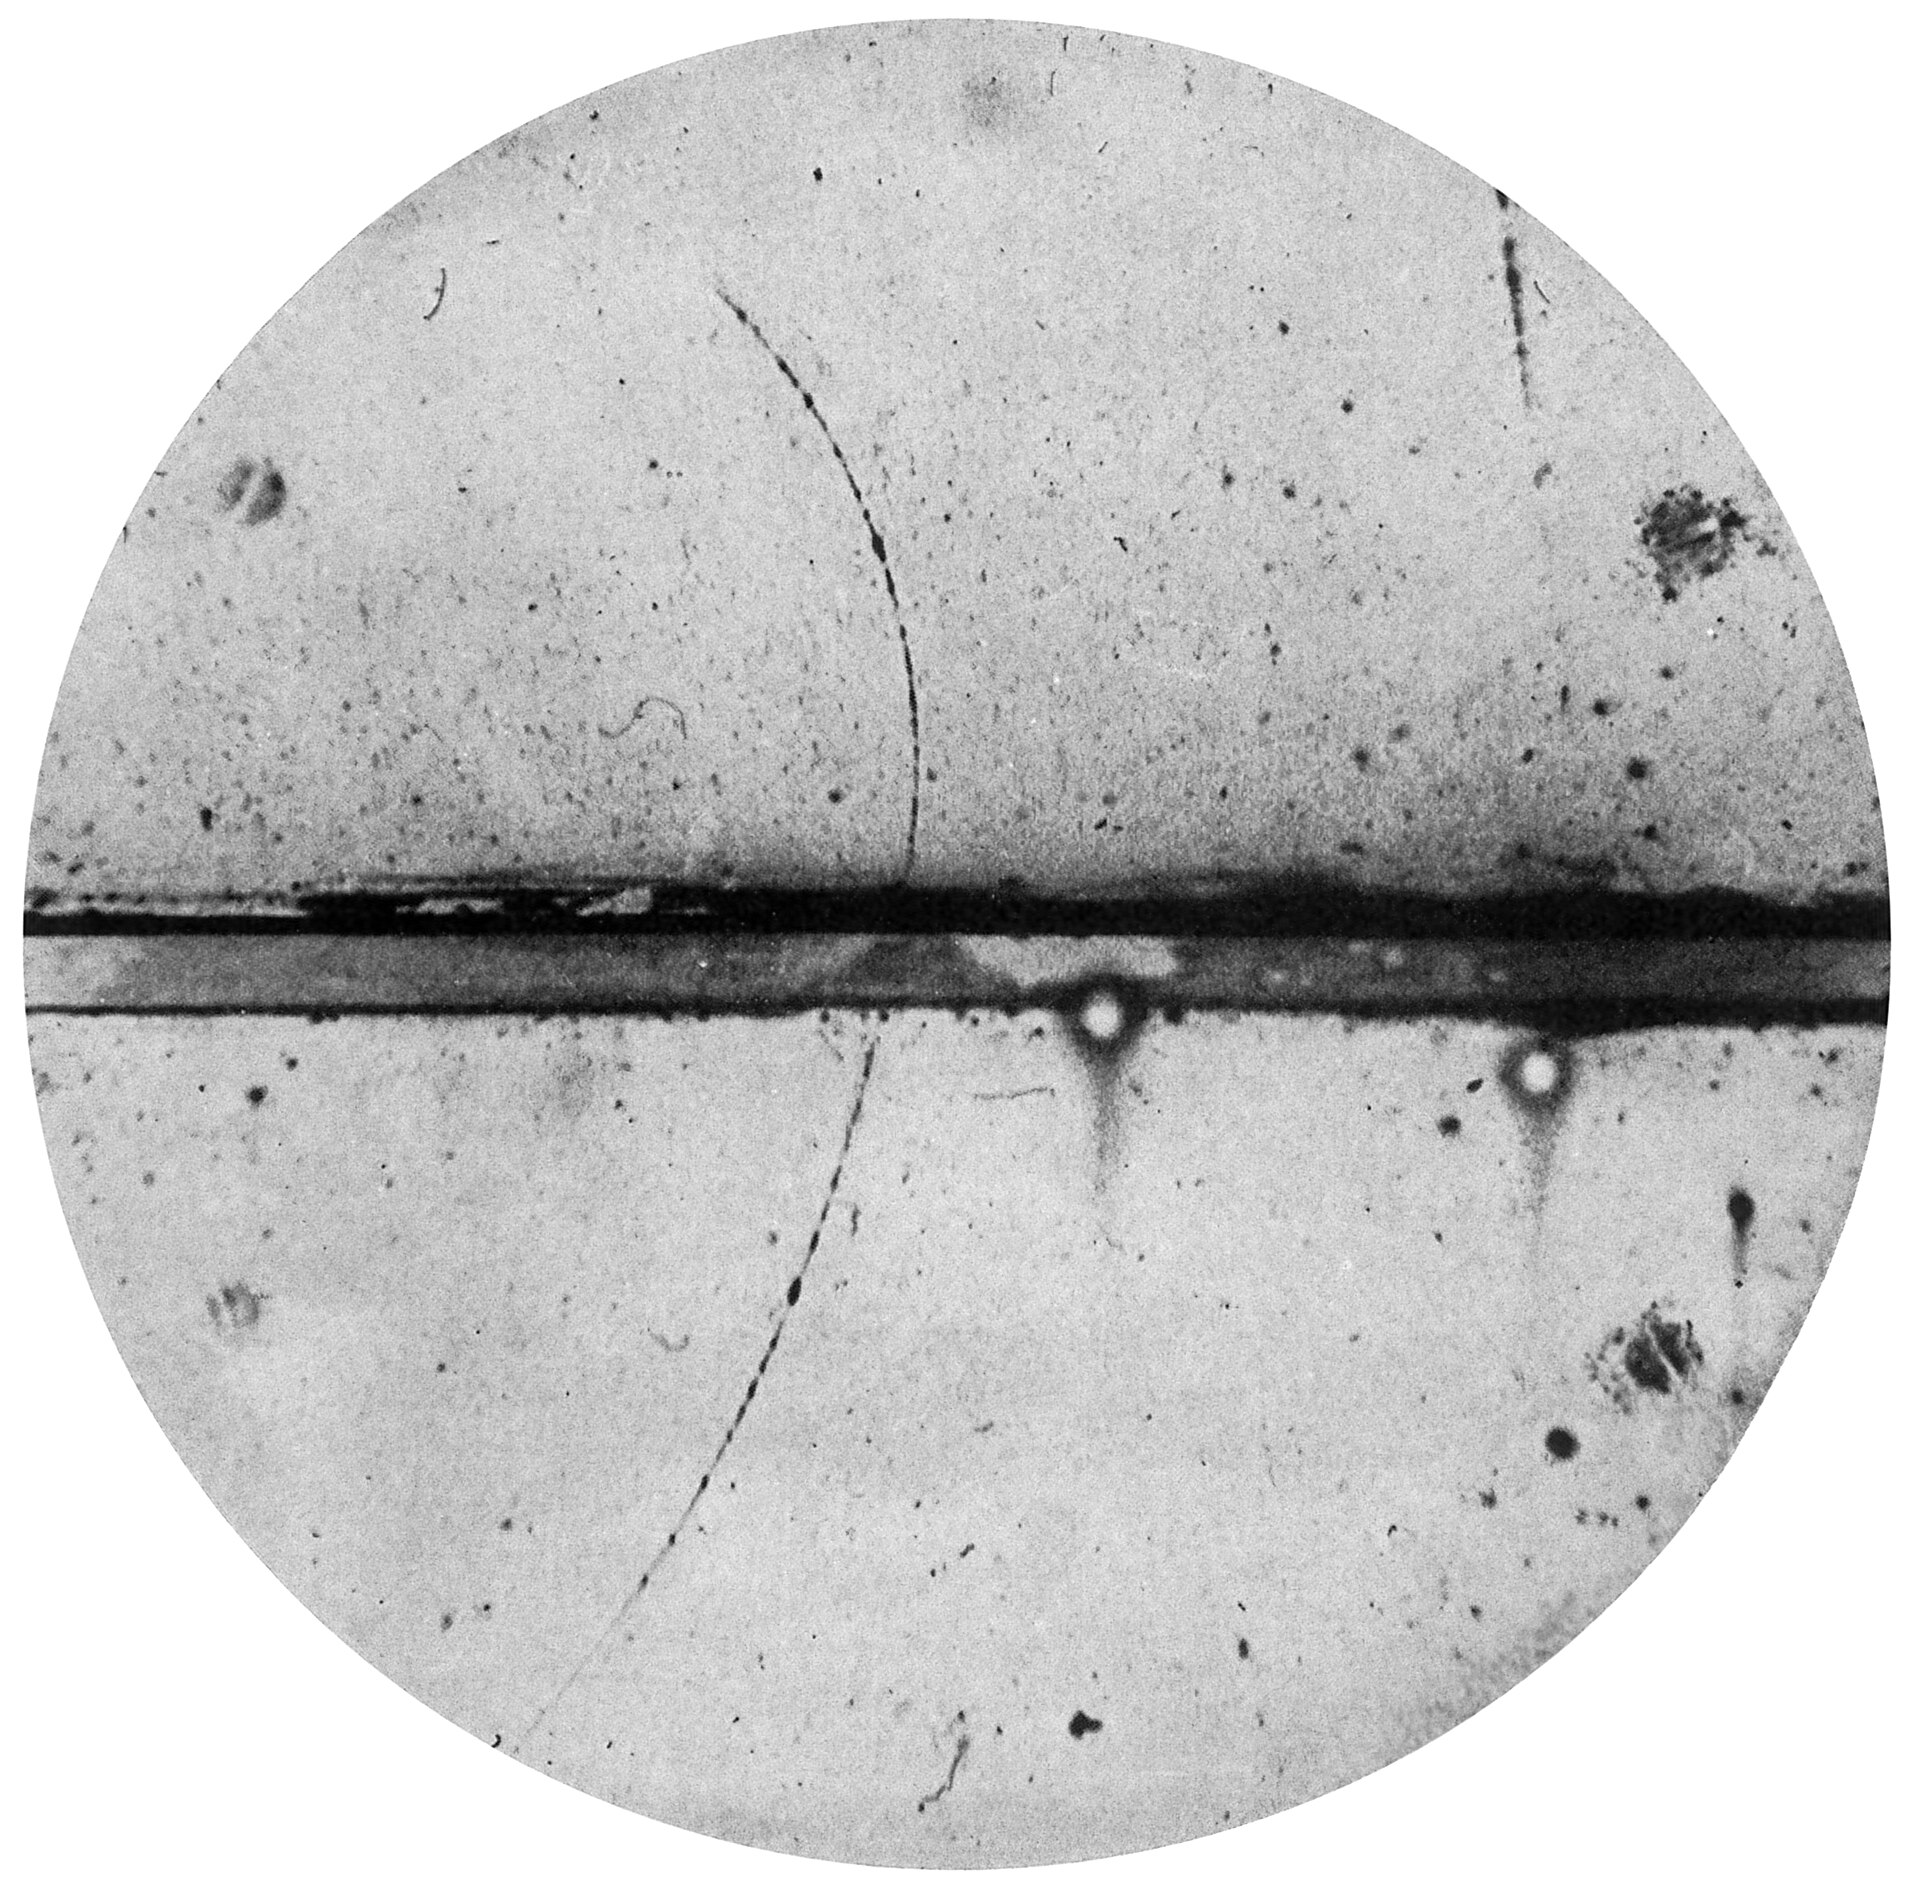
\includegraphics[width=0.5\linewidth]{images/book5/photo-positron-anderson.jpg}

{\small प्रतिपदार्थ की खोज (कार्ल एंडरसन, 1932, सार्वजनिक अधिकार-क्षेत्र): कुहरा-कक्ष की सीसे की पट्टिका से ऊपर चढ़ता एक अकेला पॉज़िट्रॉन, जो इलेक्ट्रॉन के लिए उलटी दिशा में और प्रोटॉन के लिए बहुत कसकर मुड़ा हुआ है --- $E = mc^2$ का बहीखाता उलटी दिशा में चलता हुआ पकड़ा गया।}
\end{omfigure}

\section{समस्या: पदार्थ बनाना --- प्रतिप्रोटॉन और बेवाट्रॉन}

\begin{problem}[{सप्ताहांत समस्या --- संवेग-संरक्षण ने प्रतिसंसार का
मोल कैसे तय किया}]\label{pb:b3:relativistic-dynamics:1}
1931 से डिराक के समीकरण यह माँग कर रहे थे कि प्रोटॉन का कोई विपरीत
आवेश वाला दर्पण-जुड़वाँ हो। एक बनाने का अर्थ था उसकी \omterm{def:b3:relativistic-dynamics:momentum-energy}{विराम ऊर्जा} को
पुंज-ऊर्जा से खरीदना --- और उसका मोल संवेग-संरक्षण ने तय किया। यह
समस्या वह मोल आँकती है, उसे चुकाने वाली मशीन का अभिकल्प करती है, और
1955 की खोज का पीछा करती है। आँकड़े: $m_{\text{p}}c^2 = \qty{938.3}{MeV}$;
आवेश और \emph{बैरिऑन संख्या} (प्रोटॉन और न्यूट्रॉन $+1$, प्रतिप्रोटॉन $-1$)
हर अभिक्रिया में संरक्षित रहते हैं।

\medskip\noindent\textbf{भाग I --- \omterm{def:b3:relativistic-dynamics:four-momentum}{चतुःसंवेग} की औज़ार-पेटी।}
\begin{enumerate}
  \item एक कण के लिए $E^2 - p^2c^2 = m^2c^4$ दिखाइए, $E$ और
        $\vect p$ की परिभाषाओं से।
  \item किसी निकाय के लिए $E_{\text{कुल}}^2 -
        p_{\text{कुल}}^2c^2$ सभी तंत्रों में एक ही क्यों है, और
        संवेग-केंद्र तंत्र में वह किसके बराबर है?
  \item ऊर्जा $E$ का कोई प्रोटॉन-पुंज विराम में रखे प्रोटॉन से टकराता
        है: दिखाइए कि
        $M^2c^4 = 2m_{\text{p}}^2c^4 + 2E\,m_{\text{p}}c^2$।
  \item दोनों सीमाएँ जाँचिए: नीची ऊर्जा पर $Mc^2 \to
        2m_{\text{p}}c^2$; ऊँची ऊर्जा पर $Mc^2 \approx
        \sqrt{2E\,m_{\text{p}}c^2}$ --- वही वर्गमूल-नियम।
  \item कोई अभिक्रिया तभी अनुमत है जब $Mc^2$ उत्पादों के
        विराम-द्रव्यमानों के योग तक पहुँच जाए, और देहली पर सारे उत्पाद
        संवेग-केंद्र तंत्र में विराम में हों: इस अंतिम उपवाक्य का
        औचित्य दीजिए।
  \item नियत लक्ष्य पर प्रयोगशाला में उत्पादों की गतिज ऊर्जा कण-सृजन
        के लिए कभी वापस क्यों नहीं पाई जा सकती?
\end{enumerate}

\medskip\noindent\textbf{भाग II --- प्रतिप्रोटॉन का मोल।}
\begin{enumerate}[resume]
  \item $p + p$ संघट्टों में प्रतिप्रोटॉन $\bar p$ बनाने वाली सबसे
        सस्ती अभिक्रिया को एक \emph{अतिरिक्त} प्रोटॉन भी बनाना पड़ता
        है: उसे लिखिए, और आवेश तथा बैरिऑन संख्या से औचित्य दीजिए।
  \item दिखाइए कि देहली के लिए $Mc^2 = 4m_{\text{p}}c^2$ चाहिए।
  \item आवश्यक पुंज-ऊर्जा $E = 7m_{\text{p}}c^2$ और गतिज ऊर्जा
        $T = 6m_{\text{p}}c^2$ निकालिए; $T$ का मान निकालिए।
  \item देहली पर पुंज की गतिज ऊर्जा का कितना अंश सचमुच नया
        विराम-द्रव्यमान बना (उसमें से $2m_{\text{p}}c^2$)?
        शेष कहाँ है?
  \item आमने-सामने के किसी $p$--$p$ संघट्टक में उसी अभिक्रिया को
        \emph{प्रति पुंज} कितनी गतिज ऊर्जा चाहिए? दोनों अभिकल्पों की
        तुलना कीजिए।
  \item 1954 में कोई संघट्टक नहीं था (पुंज इतने विरल थे कि आपस में
        टकरा ही नहीं पाते): किस व्यावहारिक तथ्य ने नियत-लक्ष्य वाला
        चुनाव कराया, और पुंज-ऊर्जा में उसकी क्या कीमत पड़ी?
\end{enumerate}

\medskip\noindent\textbf{भाग III --- बेवाट्रॉन का अभिकल्प।}
बर्कली में बनी मशीन $T = \qty{6.2}{GeV}$ तक पहुँची ---
देहली से आराम से ऊपर --- और उसके द्विध्रुव-क्षेत्र $B =
\qty{1.56}{T}$ थे।
\begin{enumerate}[resume]
  \item शिखर ऊर्जा पर पुंज की कुल ऊर्जा और संवेग निकालिए।
  \item मोड़-त्रिज्या $r = p/qB$ निकालिए और मशीन के \qty{15.2}{m} से
        तुलना कीजिए।
  \item प्रोटॉन की चाल और $2\pi r$ के वलय पर परिक्रमण-आवृत्ति
        निकालिए।
  \item अंतःक्षेपण पर प्रोटॉन \qty{10}{MeV} गतिज ऊर्जा के साथ आते
        हैं: उनकी चाल निकालिए, और समझाइए कि हर चक्र में त्वरक-आवृत्ति
        को \emph{झाड़ू} की तरह क्यों बदलना पड़ता था ($E$ बढ़ने के साथ
        कौन-सी दो राशियाँ बदलती हैं?)।
  \item प्रति चक्कर लगभग \qty{1.5}{kV} मिलने पर, एक त्वरण-चक्र में
        कितने चक्कर लगते हैं और कितना समय?
  \item नाम ``बेवाट्रॉन'' BeV से आया, अर्थात् अरब इलेक्ट्रॉनवोल्ट:
        एक पंक्ति में बताइए कि कौन-सी भौतिकी ने अभिकल्प का आँकड़ा
        $6$ और कुछ BeV तय किया।
\end{enumerate}

\medskip\noindent\textbf{भाग IV --- खोज, 1955।}
\begin{enumerate}[resume]
  \item कोई चुंबक हर संभावित कण को एक वृत्त पर मोड़ता है: समझाइए कि
        इससे कणों की छँटाई \emph{संवेग} से होती है ($r = p/qB$),
        ऊर्जा या चाल से नहीं --- और संवेग से छँटा पुंज फिर भी
        जातियाँ क्यों मिलाए रखता है।
  \item ताँबे के लक्ष्य पर पड़ता पुंज ऋणात्मक पायॉनों
        ($m_\pi c^2 = \qty{139.6}{MeV}$) की बाढ़ बनाता था, जिनमें
        कुछ प्रतिप्रोटॉन छिपे रहते थे। वर्णक्रममापी ने संवेग
        $p = \qty{1.19}{GeV}/c$ के ऋणात्मक कण छाँटे: उस संवेग पर किसी
        प्रतिप्रोटॉन की और किसी पायॉन की चाल निकालिए।
  \item \qty{12}{m} के उड़ान-पथ पर दोनों उड़ान-काल निकालिए: इस खोज को
        कितनी काल-विभेदन क्षमता चाहिए थी?
  \item एक दूसरी, स्वतंत्र पहचान चेरेनकोव गणकों से हुई, जो केवल किसी
        चाल-देहली से ऊपर ही चलते हैं: किस कण को उन्हें चलाने के लिए
        सजाया गया था, और किसी खोज के लिए बहुलता क्यों महत्वपूर्ण है?
  \item चेंबरलेन और सेग्रे ने प्रति $\num{44000}$ पायॉनों पर लगभग
        एक प्रतिप्रोटॉन गिना: देहली वाले तर्क ने यह क्यों सुनिश्चित
        कर रखा था कि देहली से ऊपर भी दर बहुत छोटी ही रहेगी?
  \item कोई प्रतिप्रोटॉन अंततः किसी प्रोटॉन से मिलकर विनष्ट हो जाता
        है: प्रति घटना कितनी ऊर्जा मुक्त होती है, और प्रायः किस रूप में?
  \item नामित परिणाम का सार लिखिए: \omterm{def:b3:relativistic-dynamics:four-momentum}{चतुःसंवेग} के संरक्षण ने
        प्रतिप्रोटॉन का मोल नियत लक्ष्य पर $T = 6m_{\text{p}}c^2 =
        \qty{5.6}{GeV}$ ठहराया; \qty{6.2}{GeV} के, \qty{15}{m} के
        किसी सिंक्रोट्रॉन ने वह चुकाया, और प्रतिसंसार प्रयोगशाला का
        तथ्य बन गया --- 1959 का नोबेल पुरस्कार।
\end{enumerate}
\end{problem}
